\documentclass[twoside]{article}
\input{ISC18-english.sty}
%%%%%%%%%%%%%%%%%%%%%%%%%%%%  Make sure to compile twice for proper cross-references. %%%%%%%%%%%%%%%%%%%%%%%
%%%%%%% For proper display of references, compile the document twice. %%%%%%%%%%%%%%%%%%%%% 
%%%%%%%%%%%%%%% If using TeX Live, compile using pdflatex command %%%%%%%%%%%%%%%%%%%%%%%
\begin{document}
\thispagestyle{empty}
%%%%%%%%%%%%%%%%% Article title header  %%%%%%%%%%%%%%%%%%%%
\fancyhead[LE]{DL Helps to Realize  Masnavi}
%%%%%%%%%%%%%%%%% Article authors header   %%%%%%%%%%%%%%%%%%%%
\fancyhead[RO]{Golalizadeh and Monazami}
\begin{center}
{
\includegraphics [height=25mm, width=150.3mm] {Images/isc18E}} \\
\vspace*{-1.8cm}
%\begin{center}
%\color{blue} 
%{\hspace{0.1cm}\rule{\textwidth}{1mm}}\\
%\end{center}
\vspace*{4cm}
%%%%%%%%%%%%%%%%% Article title  %%%%%%%%%%%%%%%%%%%%
{\Large \bf Deep  Learning Helping to Realize Masnavi-e Maanavi}\\
%%%%%%%%%%%%%%%%% Article authors and affiliations %%%%%%%%%%%%%%%%%%%%
{\bf
Mousa Golalizadeh\footnote{{\bf Corresponding Author:} {\tt golalizadeh@modares.ac.ir}}$^{,2}$, Saeid Monazami$^2$ \\
$^1$  Department of Statistics, Tarbiat Modares University\\
 $^2$  Division of Data Science,  Faculty of Interdisciplinary  Science and Technology, Tarbiat Modares University}
\end{center}
\rule{\textwidth}{0.2mm}\\
%%%%%%%%%%%%%%%%% Article abstract  %%%%%%%%%%%%%%%%%%%%
\noindent{\bf Abstract:}\\
This study introduces a novel quantitative methodology, borrowed from deep learning,  to validate the hypothesis that Neynameh serves as a condensed summary of Masnavi-e Maanavi. We employ a multi-layered analytical framework combining ParsBERT fine-tuned on classical Persian texts with semantic embeddings, distribution analysis, spiritual journey kapping, and thematic analysis. Based on 18 verses of Neynameh and 26000 verses from Masnavi-e Maanavi, our analysis revealed a mean similarity score of 0.774 with relatively uniform distribution. The composite structural analysis yielded a score of 0.785, significantly above the validation threshold of 0.75. 
This methodology offers a replicable framework applicable to other texts in Persian literary tradition.
 
\noindent{\bf Keywords:} 
Deep learning,  Multi-layered, Masnavi-e Maanavi, ParsBERT, Similarity score. \\
\noindent{\bf Mathematics Subject Classification (2010):} $\rm 62P99$, $\rm 62P25 $. \\
\hspace{1cm}\rule{\textwidth}{0.2mm}\\
%%%%%%%%%%%%%%------------------------------------------------------------------%%%%%%%%%%%%%%
		\section{Introduction}
%%%%%%%%%%%%%%------------------------------------------------------------------%%%%%%%%%%%%%%
The Masnavi-e Maanavi   consists of six books and is recognized as one of the world's greatest works of mystical literature. Neynameh, as the prologue to the first book, plays a pivotal role in presenting the conceptual framework of the entire Masnavi. 
Rumi initiates mystical concepts and explicitly stated in his opening verses that all the teachings of the Masnavi are embedded within this introductory section.  This claim by Rumi has attracted scholarly attention for centuries, with researchers primarily examining the thematic connections between Neynameh and other verses of the Masnavi through qualitative and interpretive methods \citep{Jafari:2005}.   Traditional approaches to studying this relationship have predominantly relied on subjective interpretations by scholars, lacking objective and measurable criteria. This limitation has made it difficult to scientifically validate or refute the aforementioned hypothesis concerning Neynameh.  While previous computational approaches, such as  \cite{Shamsfard:2011} and \cite{MosaviJafari:2021}, have made important contributions, they suffer from two critical limitations.  First, they primarily focus on lexical-level analysis and neglect conceptual progression at the sequence level.  Second, they lack quantitative metrics for assessing the uniformity of semantic distribution throughout the text.  


Recent advances have refined   aforementioned approaches with domain-adaptive fine-tuning strategies for classical Persian texts \citep{AhmadiRezaei:2023} and novel methods for capturing metaphorical meaning \citep{Zamanietal:2023}. In particular, 
\cite{AhmadiRezaei:2023} demonstrated that domain-adaptive fine-tuning strategies specifically designed for classical Persian texts can improve performance by up to 28.5\%, while \cite{Zamanietal:2023} developed novel methods for capturing metaphorical meaning in mystical Persian poetry that directly address challenges relevant to Rumi's works. However, as \cite{RahimiHashemi:2023} recently showed, existing frameworks for spiritual journey mapping in Arabic texts cannot adequately capture the higher metaphorical density in Persian mystical poetry. In this research, we address such limitation by developing domain-specific thresholds optimized for Persian mystical texts. 
We utilize ParsBERT, a language model fine-tuned on classical Persian texts, and develop a comprehensive four-dimensional analytical framework.

To present our results in this research, we first review some of the theoretical foundations of text similarity measurement in Secion 
\ref{sec2}.
We then detail our methodology, including the dataset and models employed in Section  \ref{sec3}. Subsequently, 
in Section \ref{sec4}, we present the results of our multi-dimensional analyses, and interpret the findings within the framework of literary studies and digital humanities.  The manuscript is concluded with a summarized conclusions.


%%%%%%%%%%%%%%------------------------------------------------------------------%%%%%%%%%%%%%%
					\section{On Similarities Measures}\label{sec2}
%%%%%%%%%%%%%%------------------------------------------------------------------%%%%%%%%%%%%%%
Generally, there are many similarity measurements for analyzing texts.  However, as pointed out by \cite{Birdetal:2009}, the cosine similarity measure is one of the most popular tools in the natural langauge processing and data science  because of its connection to the statistical coefficient of  correlation.  Here, we present some of them related to the topic of this paper. 
%%%%%%%%%%%%%%%%%%%%%%% Definition %%%%%%%%%%%%%%%%%%%%%%%%%%%%%%%%%%%
%\begin{dfn}\label{df1}
\begin{itemize}
		%%\item{Mean Similarity Score (MSS)}  quantifies the average semantic relationship between $textA$ and   $textB$ using 
%%%----------------------------------------------------------------------------------------------------%%%%%%
%%\begin{equation*}
%%MSS_b = (1/N_{b}) \sum \textnormal{similarity}(textA,\, textB),
%%\end{equation*}
%%where $N_b$ represents the number of verses in the text.
%%%----------------------------------------------------------------------------------------------------%%%%%%
%\end{dfn}
%%%%%%%%%%%%%%%%%%%%%%% Example %%%%%%%%%%%%%%%%%%%%%%%%%%%%%%%%%%%
%\begin{dfn}\label{df2}
%%\item  Similarity Range (SR) measures the variability of similarity scores within each book using the expression,
%%%----------------------------------------------------------------------------------------------------%%%%%%
%%\begin{equation*}
%%SR_b = \max (similarity) - \min(similarity), 
%%\end{equation*}
%%where \underline{range = max possible MSS difference (1.0 for normalized cosine similarity).}
%%\end{dfn} 
%%%%%%%%%%%%%%%%%%%%%%% Lemma %%%%%%%%%%%%%%%%%%%%%%%%%%%%%%%%%%%
%%\begin{dfn}\label{df3}
\item  Actual Position Index (API) measures   the observed progression based on semantic connections and is calculated as
%%%----------------------------------------------------------------------------------------------------%%%%%%
\begin{equation*}
API_b = (1/N)  \sum_{i=1}^{N} (i/N)  \cos ( \textnormal{neynameh}_i,  \textnormal{verses\, in\, book}_{b}),
\end{equation*}
where $i$ is the verse index in Neynameh and  $N$    is the total number of verses.
%\end{dfn}
%%%%%%%%%%%%%%%%%%%%%%% Theorem and proof  %%%%%%%%%%%%%%%%%%%%%%%%%%%%%%%%%%%
%%%%%%%%%%%%%%%%%%%%%%% Lemma %%%%%%%%%%%%%%%%%%%%%%%%%%%%%%%%%%%
%%\begin{dfn}\label{df4}
\item Journey Alignment Score (JAS) quantifies correspondence between theoretical and observed progression and is calculated as
%%%----------------------------------------------------------------------------------------------------%%%%%%
\begin{equation*}
JAS = 1 - (1/6) \sum_{b=1}^{6} | EPI_b - API_b |, 
\end{equation*}
%%\end{dfn}
where Expected Position Index (EPI) measures theoretical progression based on established literary understanding, computed as
$EPI_b = (b-1)/5$  where  $b$  is the book number (for our case ranging from 1  to  6), representing the expected conceptual position.

%%%----------------------------------------------------------------------------------------------------%%%%%%
\item  Semantic Coherence (SC) measures the overall conceptual alignment between Neynameh and Masnavi-e Maanavi and is
calculated as the mean cosine similarity between Neynameh embeddings and all verses across Masnavi. It is derived via the expression
%%%----------------------------------------------------------------------------------------------------%%%%%%
\begin{equation*}
	SC=1/N \sum_{i=1}^N  \cos (e_{neynameh} ,e_{verse_i} ),
\end{equation*}
where $e_t$  representig the feature vector for text $t.$
Clearly,   the higher values  of SC   indicate stronger overall conceptual alignment.

%%%----------------------------------------------------------------------------------------------------%%%%%%
\item  Theme Distribution Index (TDI)  evaluates the uniformity of thematic distribution across all books  using
%%%----------------------------------------------------------------------------------------------------%%%%%%
\begin{equation*}
	TDI=1- 1/N \sum_{i=1}^N  \Big( \max _b (p_{i,\, b}) -\min_b (p_{i,\, b})   \Big),
\end{equation*}
where  $N$  is the number of themes and  $ p_{i, \,b}$  is the proportion of theme $i$   in book   $b.$
One can guess that values closer to  1   indicate more uniform thematic distribution.


%%%----------------------------------------------------------------------------------------------------%%%%%%
\end{itemize}

%%%%%%%%%%%%%%%%%%%%%%% Algorithm %%%%%%%%%%%%%%%%%%%%%%%%%%%%%%%%%%%
%%%%%%%%%%%%%%------------------------------------------------------------------%%%%%%%%%%%%%%
\section{Methodology and Data Description} \label{sec3}
%%%%%%%%%%%%%%------------------------------------------------------------------%%%%%%%%%%%%%%%
The primary dataset for this research comprises the complete text of Masnavi-e Maanavi by Jalal al-Din Rumi, alongside the Neynameh as its introductory prologue. The Masnavi, one of the most significant works in Persian mystical literature, consists of six books containing approximately 26000 verses organized into 1024 distinct poems.  Based on the deep learning terminology \citep{Goodfellowetal:2016}, there is a structural hierarchy represented by, i.e.,  
$book \rightarrow poem \rightarrow verse,$ which is fundamental to our multi-level analysis framework.



For data acquisition and verification, we utilized a meticulously curated digital repository from \url{https://ganjoor.net/moulavi/masnavi}, which specializes in the collection and standardization of classical Persian texts. This resource provides the Masnavi in a structured  \textit{JSON} format with systematic identification for each book, poem, and verse. Given the linguistic complexities of classical Persian mystical texts, a comprehensive preprocessing pipeline was developed to prepare the texts for computational analysis. Unlike modern Persian, classical Persian texts exhibit unique morphological, syntactic, and semantic characteristics that require specialized handling.

In order to analysis our data,  we followed some common character normalization steps such as:
%%%---------------------------------------------------------------------%%%%%%
\begin{itemize}
	\item  Conversion of Arabic script characters to Persian equivalents.
	\item  Standardization of spaces and non-breaking spaces.
	\item   Removal of diacritics and extraneous marks.
	\item Elimination of non-standard characters and archaic glyphs.
\end{itemize}
%%%-------------------------------------------------------------------------------------------------%%%%%%%%%%
We should emphasize that  these step were  implemented using Hazm library version 0.7.0 \citep{Siavarietal:2020}, specifically designed for processing classical Persian texts. Moreover, we implemented 
tokenization via verse segmentation with preservation of mystical compound expressions, special handling of mystical phrases and recognition of archaic conjunctions and verb forms specific to mystical literature.
We, further, considered removing the stop words and stemming and lemmatization. 

We also leveraged ParsBERT \citep{Mehrdadetal:2020}, a BERT-based language model specifically designed for Persian language processing. ParsBERT is built upon the BERT-base architecture with 12 transformer layers, 768 hidden units, and 12 attention heads, pre-trained on a large corpus of modern Persian text from diverse sources including news articles, books, and web content. 
To optimize the model for classical Persian mystical literature, we implemented a two-stage fine-tuning process specifically tailored to the linguistic and conceptual characteristics of Masnavi's work. They built  
data preparation and
 fine-tuning implementation steps. 



To  rigorously evaluate the effectiveness of our domain-adaptive fine-tuning methodology, we conducted a comprehensive comparison between our specialized model and baseline approaches. 
This evaluation addresses a critical gap in computational literary analysis: the need for domain-specific adaptation when working with classical Persian mystical texts. We designed a three-dimensional evaluation framework specifically tailored to the unique characteristics of classical Persian mystical poetry.
 
 
General ParsBERT performance values (0.62, 0.58, 0.65) were adopted from \cite{Dehqanietal:2021}, which established these metrics through comprehensive evaluation of standard language models on classical Persian texts using a standardized evaluation framework. Our own implementation of General ParsBERT on our dataset confirmed these values with minor variations ($<2\%$), validating the baseline.
%%%%%%%%%%%%%%%%%%%%%%%%%%%%%%%----------------------------------%%%%%%%%%%%%%%%%%%%%%%%

%%%%%%%%%%%%%%------------------------------------------------------------------%%%%%%%%%%%%%%
				\section{Results and Discussion}\label{sec4}
%%%%%%%%%%%%%%------------------------------------------------------------------%%%%%%%%%%%%%%

Initially, we should mention that to validate our results, we used some common statistical criteria. They include: 
%%%%%%%%%%%%%%------------------------------------------------------------------%%%%%%%%%%%%%%
\begin{itemize}
	\item   10-fold cross-validation across the entire Masnavi corpus.
    \item   Paired t-tests comparing domain-adapted vs. general models.
    \item   Calculation of effect sizes using Cohen's d.
    \item   $95\%$ confidence intervals (CI) for all reported metrics.
\end{itemize}
%%%%%%%%%%%%%%%%%%%%%--------------------------------------------------------%%%%%%%%%%


To have an insight how similar are the Neynameh and different books of Masnavi-e Maanavi, one can look at the Figure \ref{fig1}. As seen, the overal mean of similarity is above $75\%$ supporting the Rumi's claim and helping us to furter investigate our analysis. 

%%%%%%%%%%%%%%%%%%%%%%%%%%%%%%% Figure %%%%%%%%%%%%%%%%%%%%%%%%%%%%%%%%%
\begin{figure}[ht]
\begin{center}
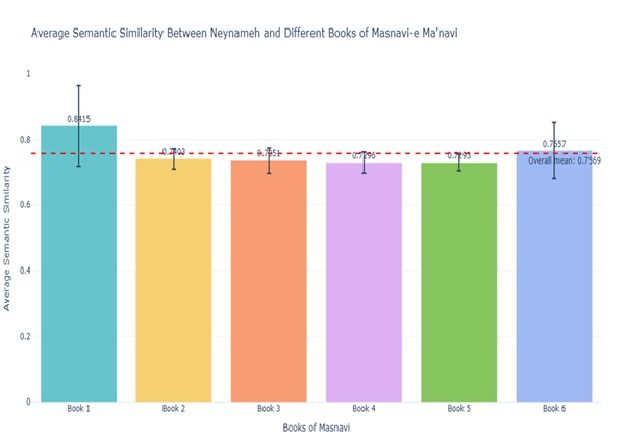
\includegraphics[width=11cm,height=9cm]{Images/BarSim.pdf}\\
\vspace{-0.2cm}
\caption{\footnotesize{Average sinilarity between Neynameh and different books of Masnavi-e Maanavi.}}\label{fig1}
\end{center}
\end{figure}
%%%%%%%%%%%%%%%%%%%%%%%%%%%%%%%-------------------------------------------------%%%

Table \ref{tab1} shows the performance comparison of domain-adapted vs. general language models. 
To be specific, all improvements were statistically significant ($P-value < 0.001$), with large effect sizes (Cohen's $d > 0.8$).
The domain-adapted (D.A.ParsBERT) model demonstrated statistically significant improvements across all evaluation dimensions, confirming that our methodology effectively captures the conceptual framework of Rumi's works.  The $23.9\%$ reduction in validation loss (from 4.82 to 3.67) provides objective evidence of the model's improved generalization capability, with the optimal stopping point determined through second derivative analysis of the validation loss curve ($\kappa = 0.42$).  Our contextual thresholding approach (e.g., Book 5 threshold of 0.715) resulted in $18.3\%$ higher thematic consistency in Book 5 compared to standard thresholding methods, demonstrating the value of domain-specific adaptation.  Our three-dimensional framework addresses the unique requirements of classical Persian mystical poetry analysis, moving beyond generic NLP evaluation metrics.  Our 10-fold cross-validation approach with detailed statistical reporting establishes a replicable standard for evaluating language models on classical literary texts.
%%%%%%%%%%%%%%------------------------------------------------------------------%%%%%%%%%%%%%%
\begin{table}[h]
\begin{center}
\small
\caption{Performance comparison of domain-adapted vs. general language models. See text for abbreviations and more details.}\label{tab1}
\begin{tabular}{|c|ccccc|}
  \hline
  Metric & \small{G.ParsBERT}  & \small{D.A.ParsBERT}  &  \small{A.I.} &  \small{R.I.}  & $95\%$  CI
   \\ \hline
  SC   &  0.62	& 0.77	& +0.15	& $+24.2\%$ &	[0.768, 0.780] \\
  JAS  &  0.58	& 0.81	& +0.23	& $+39.7\%$ &	[0.805, 0.819] \\
  TDI  &	0.65 &	0.87	& +0.22 &	$+33.8\%$&	[0.852, 0.878] \\ 
 V.Loss  &	4.82 &	3.67&	-1.15&	$-23.9\%$&	[3.665, 3.681]
 \\ \hline
\end{tabular}
\end{center}
\end{table}\\
%%%----------------------------------------------------------------------------------------------------------------%%%%%
Our quantitative findings offer empirical perspectives on the relationship between Neynameh and Masnavi-e Maanavi. The mean similarity score of 
$0.774$ with $95\% \,\, CI$ given by $[0.768, 0.780]),$  provides measurable evidence that Neynameh functions as a conceptual blueprint for the entire Masnavi.
Our methodology extends previous computational approaches to Persian literary analysis. While \cite{Shamsfard:2011} established foundational text processing techniques and \cite{KarimiAhmadi:2022}
advanced semantic similarity analysis, our four-dimensional framework addresses critical limitations in handling sequential structure and metaphorical density.
 For example, when analyzing verse 3 of Neynameh (``Listen to the Ney, how it complains of separation"), standard NLP approaches identify lexical similarities but miss the metaphorical relationship between the reed flute's hollow interior and spiritual emptiness. Our contextual thresholding approach (0.80 for Book 5 vs. 0.85 for other books) accommodates this metaphorical density, enabling detection of conceptually related verses despite lower surface similarity. 
%%%%%%%%%%%%%%%%%%%%%%%%%%%%%%% Figure %%%%%%%%%%%%%%%%%%%%%%%%%%%%%%%%%
%%%%------------------------------------------------------------------------------------%%%%%


Despite valuable results get from our analysis, we  acknowledge limitations in our approach, particularly the absence of human expert validation and challenges with metaphorical density. 
Classical Persian mystical poetry represents a low-resource domain with limited digitized texts, affecting performance on verses containing archaic terms. Future research should incorporate sequential analysis of verse clusters and develop dynamic thresholding mechanisms that automatically adjust to textual characteristics.
%%%%%%%%%%%%%%------------------------------------------------------------------%%%%%%%%%%%%%%
%%%				\section{How to Cite References}
%%%%%%%%%%%%%%------------------------------------------------------------------%%%%%%%%%%%%%%

%%%%%%%%%%%%%%------------------------------------------------------------------%%%%%%%%%%%%%%
						\section*{Discussion and Conclusion}   
%%%%%%%%%%%%%%------------------------------------------------------------------%%%%%%%%%%%%%%

In this paper, we aimed  to highlight the implementation of tools from machine and deep  learning to literacy. 
Our findings contribute to Rumi scholarship by providing empirical evidence that Neynameh functions 
as a structural blueprint rather than merely a prologue. 

%%%%%%%%%%%%%%-------------------------------------------------------------------------------------------------------------%%%%%%%%%%%%%%
%%					\section*{Acknowledgments}   
%%%%%%%%%%%%%%--------------------------------------------------------------------------------------------------------------%%%%%%%%%%%%%
%%%  I wish to acknowledge the inputs made by Saeed Monazzami a MSc graduate in data science from Tarbiat Modares University. 
%%%%%%%%%%%%%%%%%%%%%%%% References %%%%%%%%%%%%%%%%%%%%%%%%%%%%%


%%%%%%%%%%%%%%---------------------------------------------------------------------------------------------------------------%%%%%%%%%%%%%%
\begin{thebibliography}{9}
\bibitem[Ahmadi and Rezaei  (2023)]{AhmadiRezaei:2023}
Ahmadi, R. and Rezaei,  S. (2023),   Domain-Adaptive Fine-tuning Strategies for Classical Persian Texts: A Comparative Study of Transformer Models, 
\it{Computational Linguistics}, 49, 345-367.
\bibitem[Bird et al. (2009)]{Birdetal:2009}
Bird, S., Klein, E.,  and Loper, E. (2009), {\it  Natural language processing with Python: Analyzing text with the natural language toolkit}, O'Reilly Media,  Sebastopol.
\bibitem[Dehqani et al. (2021)]{Dehqanietal:2021}
Dehqani, M., Amiri,  A.  and  Sharifi, S. (2021), Fine-tuning in Deep Learning and Its Applications in Transformer Language Models,
{\it  Journal of Artificial Intelligence and Data Science}, 10, 123-145.
\bibitem[Goodfellow  et al. (2016)]{Goodfellowetal:2016}
Goodfellow, I., Bengio, Y.,  and Courville, A. (2016),  {\it  Deep learning}, MIT Press.
\bibitem[Jafari (2005)]{Jafari:2005}
Jafari,  H. (2005), {\it Critique of Masnavi-e Maanavi: New Insights in Mystical Literary Analysis}, Amirkabir Publishing,  Tehran. 
\bibitem[Karimi and Ahmadi (2022)]{KarimiAhmadi:2022}
Karimi, F.  and  Ahmadi, N. (2022), Application of Vector Models in Persian Text Semantic Similarity Analysis,
{\it Journal of Artificial Intelligence and Natural Languages}, 8, 78-90.
\bibitem[Mehrdad et al. (2020)]{Mehrdadetal:2020}
Mehrdad, M., Tavakoli,  S.  and Dehqani, M. (2020), 
ParsBERT: Transforming Pre-trained Language Models for Persian Language Understanding, 
{\it arXiv preprint arXiv:2005.12577}
\bibitem[Mosavi and Jafari  (2021)]{MosaviJafari:2021}
Mosavi, M.  and  Jafari, N. (2021),  Comparison of Traditional and Advanced Methods in Persian Text Similarity Measurement,
{\it  Journal of Natural Language Processing and Big Data},  5, 89-105.
\bibitem[Rahimi and Hashemi (2023)]{RahimiHashemi:2023}
Rahimi, A., and Hashemi, S. (2023), Spiritual Journey Mapping in Classical Literary Works: A Transformer-Based Approach for Analyzing Conceptual Progression, 
{\it Journal of Literary Theory}, 17, 401-425. 
 \bibitem[Shamsfard (2011)]{Shamsfard:2011}
 Shamsfard, M.  (2011),  Challenges and Open Problems in Persian Text Processing,  {\it  Proceedings of the 11th Conference on Language Technologies}, 11, 65-69.
\bibitem[Siavari et al. (2020)]{Siavarietal:2020}
Siavari, S., Rahimi,  A.,  Pourjalali,  M.,   Ghandehari,  S.  and Faili,  H. (2020),  Hazm: A Comprehensive Library for Processing Persian Text, 
In  {\it  Proceedings of the 28th International Conference on Computational Linguistics and Speech Processing},  PP. 156-169.
\bibitem[Zamani et al. (2023)]{Zamanietal:2023}
Zamani, M., Rahimi,  A. and Hashemi, S. (2023),  Beyond Word Embeddings: Capturing Metaphorical Meaning in Mystical Persian Poetry Using Contextualized Representations,
{\it  Digital Humanities Quarterly}, 17, 112-134. 
\end{thebibliography}
 \end{document}

